\chapter{ベンチマーク}
\label{chap_Results}

\section{環境}

ベンチマークの実行環境を,
表\ref{table_env}に示す.

\begin{table}[hbtp]
  \label{table_env}
  \begin{center}
    \caption{実行環境}
    \begin{tabular}{cc} \hline
      Component & Type \rule[0pt]{0pt}{0pt} \\ \hline
      CPU & AMD Ryzen7 1700 (8Cores/16Threads) \rule[0pt]{0pt}{0pt} \\ 
      & Base Clock 3GHz / Max Boost Clock 3.7GHz \rule[0pt]{0pt}{0pt} \\
      & Total L1 Cache: 768KB / Total L2 Cache: 4MB / Total L3 Cache: 16MB \\
      Memory & DDR4-2666 32GB \rule[0pt]{0pt}{0pt} \\
      OS & Ubuntu 16.04 LTS \rule[0pt]{0pt}{0pt} \\
      Compiler & gcc version 5.4.0 20160609 (Ubuntu 5.4.0-6ubuntu1~16.04.11) \rule[0pt]{0pt}{0pt} \\ \hline
    \end{tabular}
  \end{center}
\end{table}


%\section{IpCHashT の測定条件}
\section{各ハッシュテーブルの概要と測定条件}
各ハッシュテーブルの key と value に uint64 型を指定して測定する.
テーブルごとの設定を次に示す.
\leavevmode \newline

%
{\bf std::unordered\_map<uint64,uint64>}

C++ の標準ライブラリに収録されているハッシュテーブル.
\leavevmode \newline

%
{\bf sstd::CHashT<uint64,uint64>}

``Separate chaining with list head cells''
\footnote{``Separate chaining with linked lists'' がテーブルにポインタしか持たず,
ポインタで接続した先から初めて key-value ペアを持つのに対して,
``Separate chaining with list head cells'' ではテーブルにも key-value ペアを内包する.} の実装の一つ.
アルゴリズム比較用のサンプル実装として,
最もシンプルなハッシュテーブルアルゴリズムの一つを選択した.
本実装では,
テーブルサイズを 2 のべき乗とし,ハッシュ値の下位ビットをテーブル番号とする.
全要素数がテーブルサイズを超える場合に,リハッシュする.
\leavevmode \newline

%
{\bf sstd::IpCHashT<uint64,uint64> (as uint8 and maxLF50)}

提案アルゴリズムの実装の一つ.
uint8 により linked list を構成する.
Load factor の最大値を 50 \% に制限している.
テーブルサイズを 2 のべき乗とし,ハッシュ値の下位ビットをテーブル番号とする.
{\rm bench.hpp} 内で {\rm iHashT\_u8h} の別名により定義されている.
\leavevmode \newline

%
{\bf sstd::IpCHashT<uint64,uint64> (as uint8 and maxLF100)}

提案アルゴリズムの実装の一つ.
uint8 により linked list を構成する.
Load factor に制限はなく,link 距離が uint8 の幅を超えるか,テーブルが全て埋まるまで要素を挿入する.
テーブルサイズを 2 のべき乗とし,ハッシュ値の下位ビットをテーブル番号とする.
{\rm bench.hpp} 内で {\rm iHashT\_u8} の別名により定義されている.
\leavevmode \newline

%
{\bf sstd::IpCHashT<uint64,uint64> (as uint16 and maxLF100)}

提案アルゴリズムの実装の一つ.
uint16 により linked list を構成する.
Load factor に制限はなく,link 距離が uint16 の幅を超えるか,テーブルが全て埋まるまで要素を挿入する.
テーブルサイズを 2 のべき乗とし,ハッシュ値の下位ビットをテーブル番号とする.
{\rm bench.hpp} 内で {\rm iHashT\_u16} の別名により定義されている.
\leavevmode \newline

%
{\bf google::dense\_hash\_map<uint64,uint64>}

Quadratic probing の実装の一つ.
メモリ効率が高く,探査速度が速い一方,
key 値の一つを空マークに,削除を行う場合はもう一つを削除マークとして予約する必要がある.
予約された値は,key 値として使用できない.
予約には,set\_empty\_key() 関数と set\_deleted\_key() 関数を用いる.
テーブルサイズを 2 のべき乗とし,ハッシュ値の下位ビットをテーブル番号とする.
\leavevmode \newline

%
{\bf ska::flat\_hash\_map<uint64,uint64,ska::power\_of\_two\_std\_hash<uint64>>}

Robin Hood Hashing の実装の一つ.
ska::power\_of\_two\_std\_hash<uint64> オプションにより,
テーブルサイズを 2 のべき乗とし,ハッシュ値の下位ビットをテーブル番号としている.

\leavevmode \newline


\section{結果}

{\bf Loadfactor}

{\bf メモリ使用量}

{\bf 挿入}

{\bf 探査}

{\bf 削除}

\begin{figure}[h]
  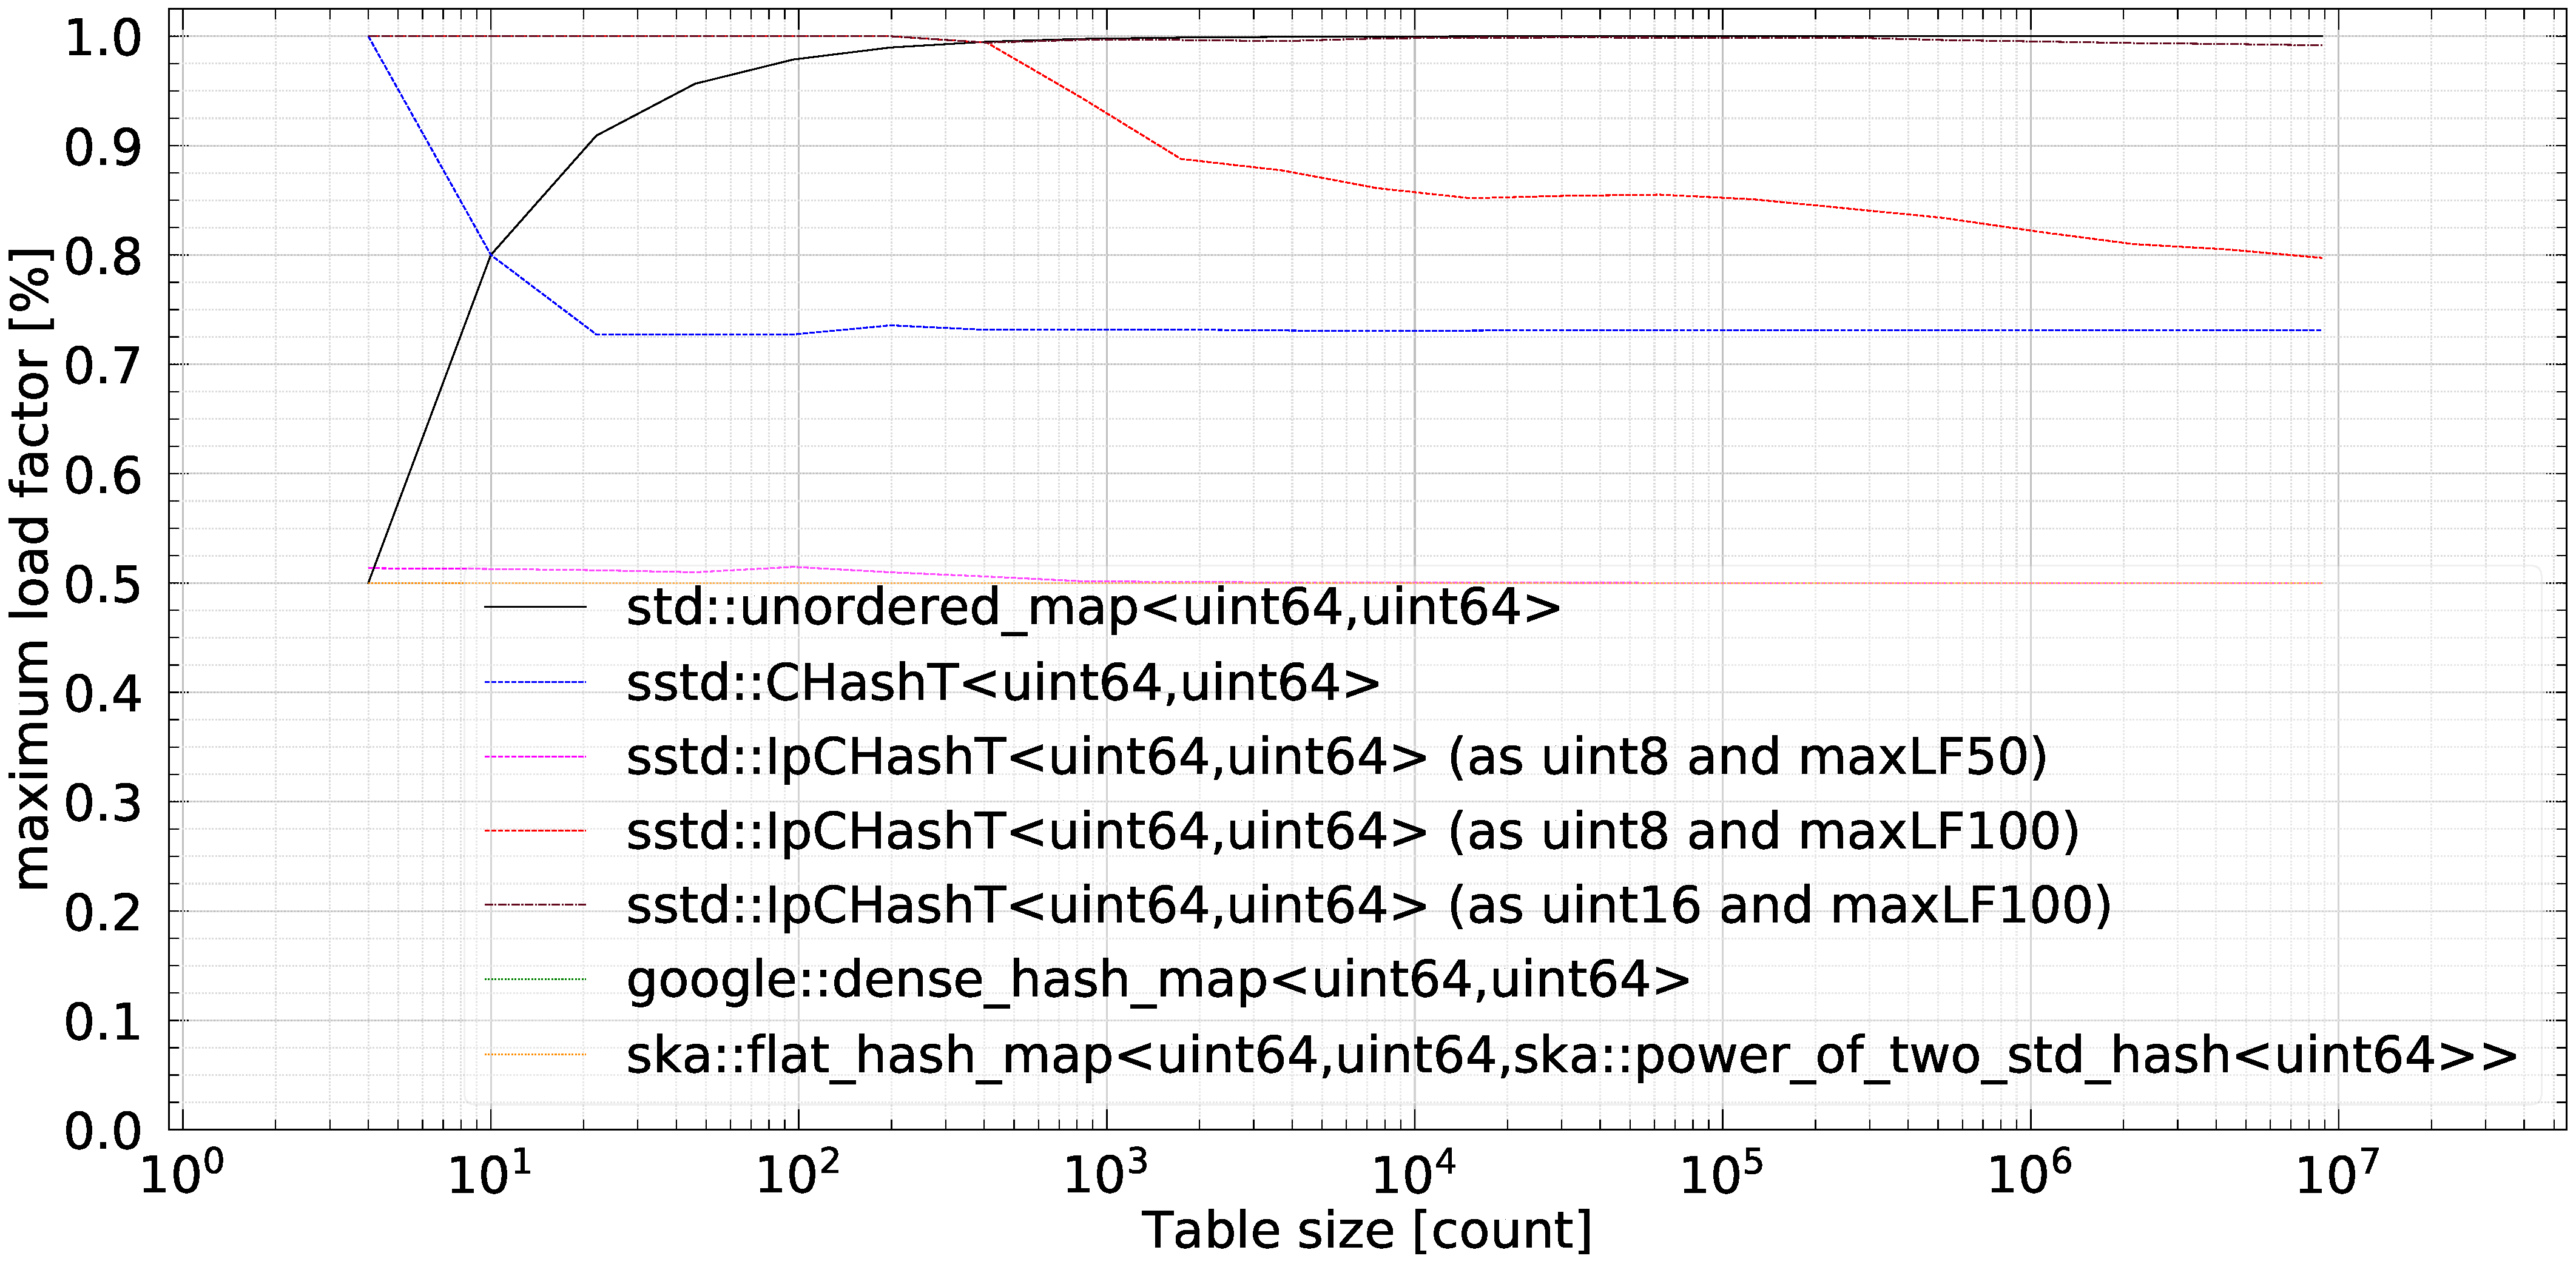
\includegraphics[scale=0.24]{./fig_bench/maxLoadFactor_med.pdf}
  \caption{
    Maximum load factor which is median value of 100 samples.
    Maximum load factor of std::IpHashT (as maxLF100) is limitted by its maximum length of shift\_T.
    Maximum load factor of std::IpHashT (as maxLF50), google::dense\_hash\_map and ska::flat\_hash\_map is artificially limited by 50 \%.
  }
  \label{fig_bench_LF}
\end{figure}

\begin{figure}[h]
  \hspace{-1mm}
  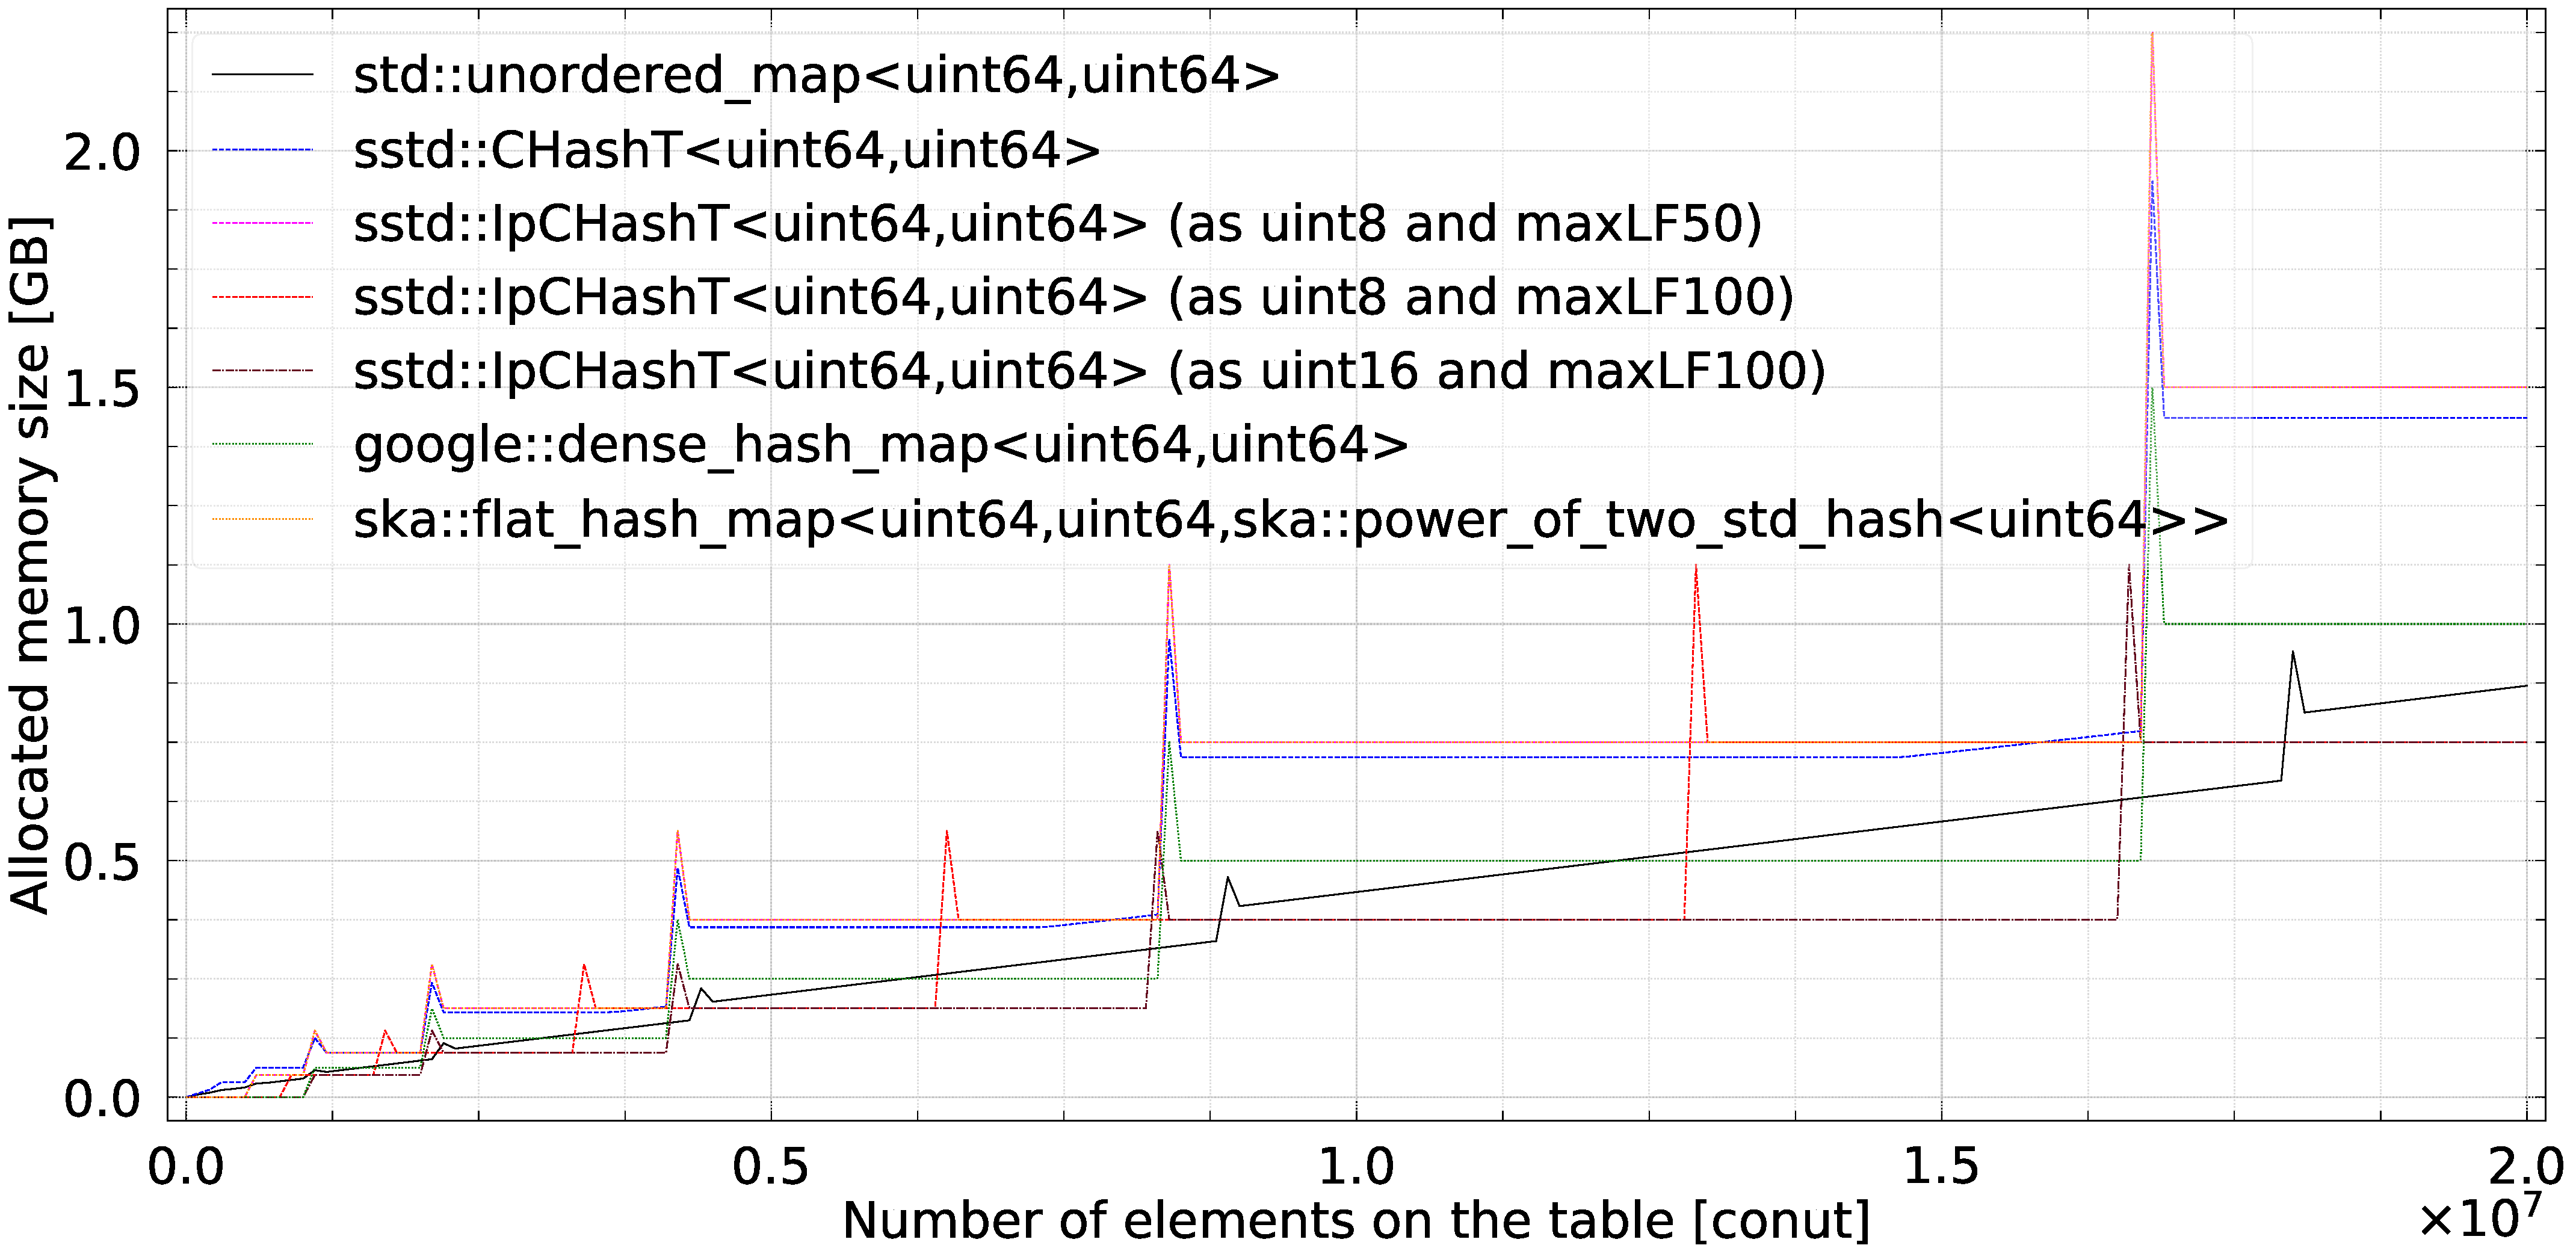
\includegraphics[scale=0.24]{./fig_bench/usedMemory.pdf}
  \caption{
    Allocated memory size which is one sample raw data.
    Peaks of memory size indicate rehash timmings.
    And the width of peaks is measurement interval.
    This means that the actual waveform is more sharp.
    std::unordered\_map seems to allocating memory each by insertion.
    sstd::IpCHashTs are moved the timming of rehashing back and forth by the influence of maximum load factor.
  }
  \label{fig_bench_memory}
\end{figure}

\begin{figure}[h]
  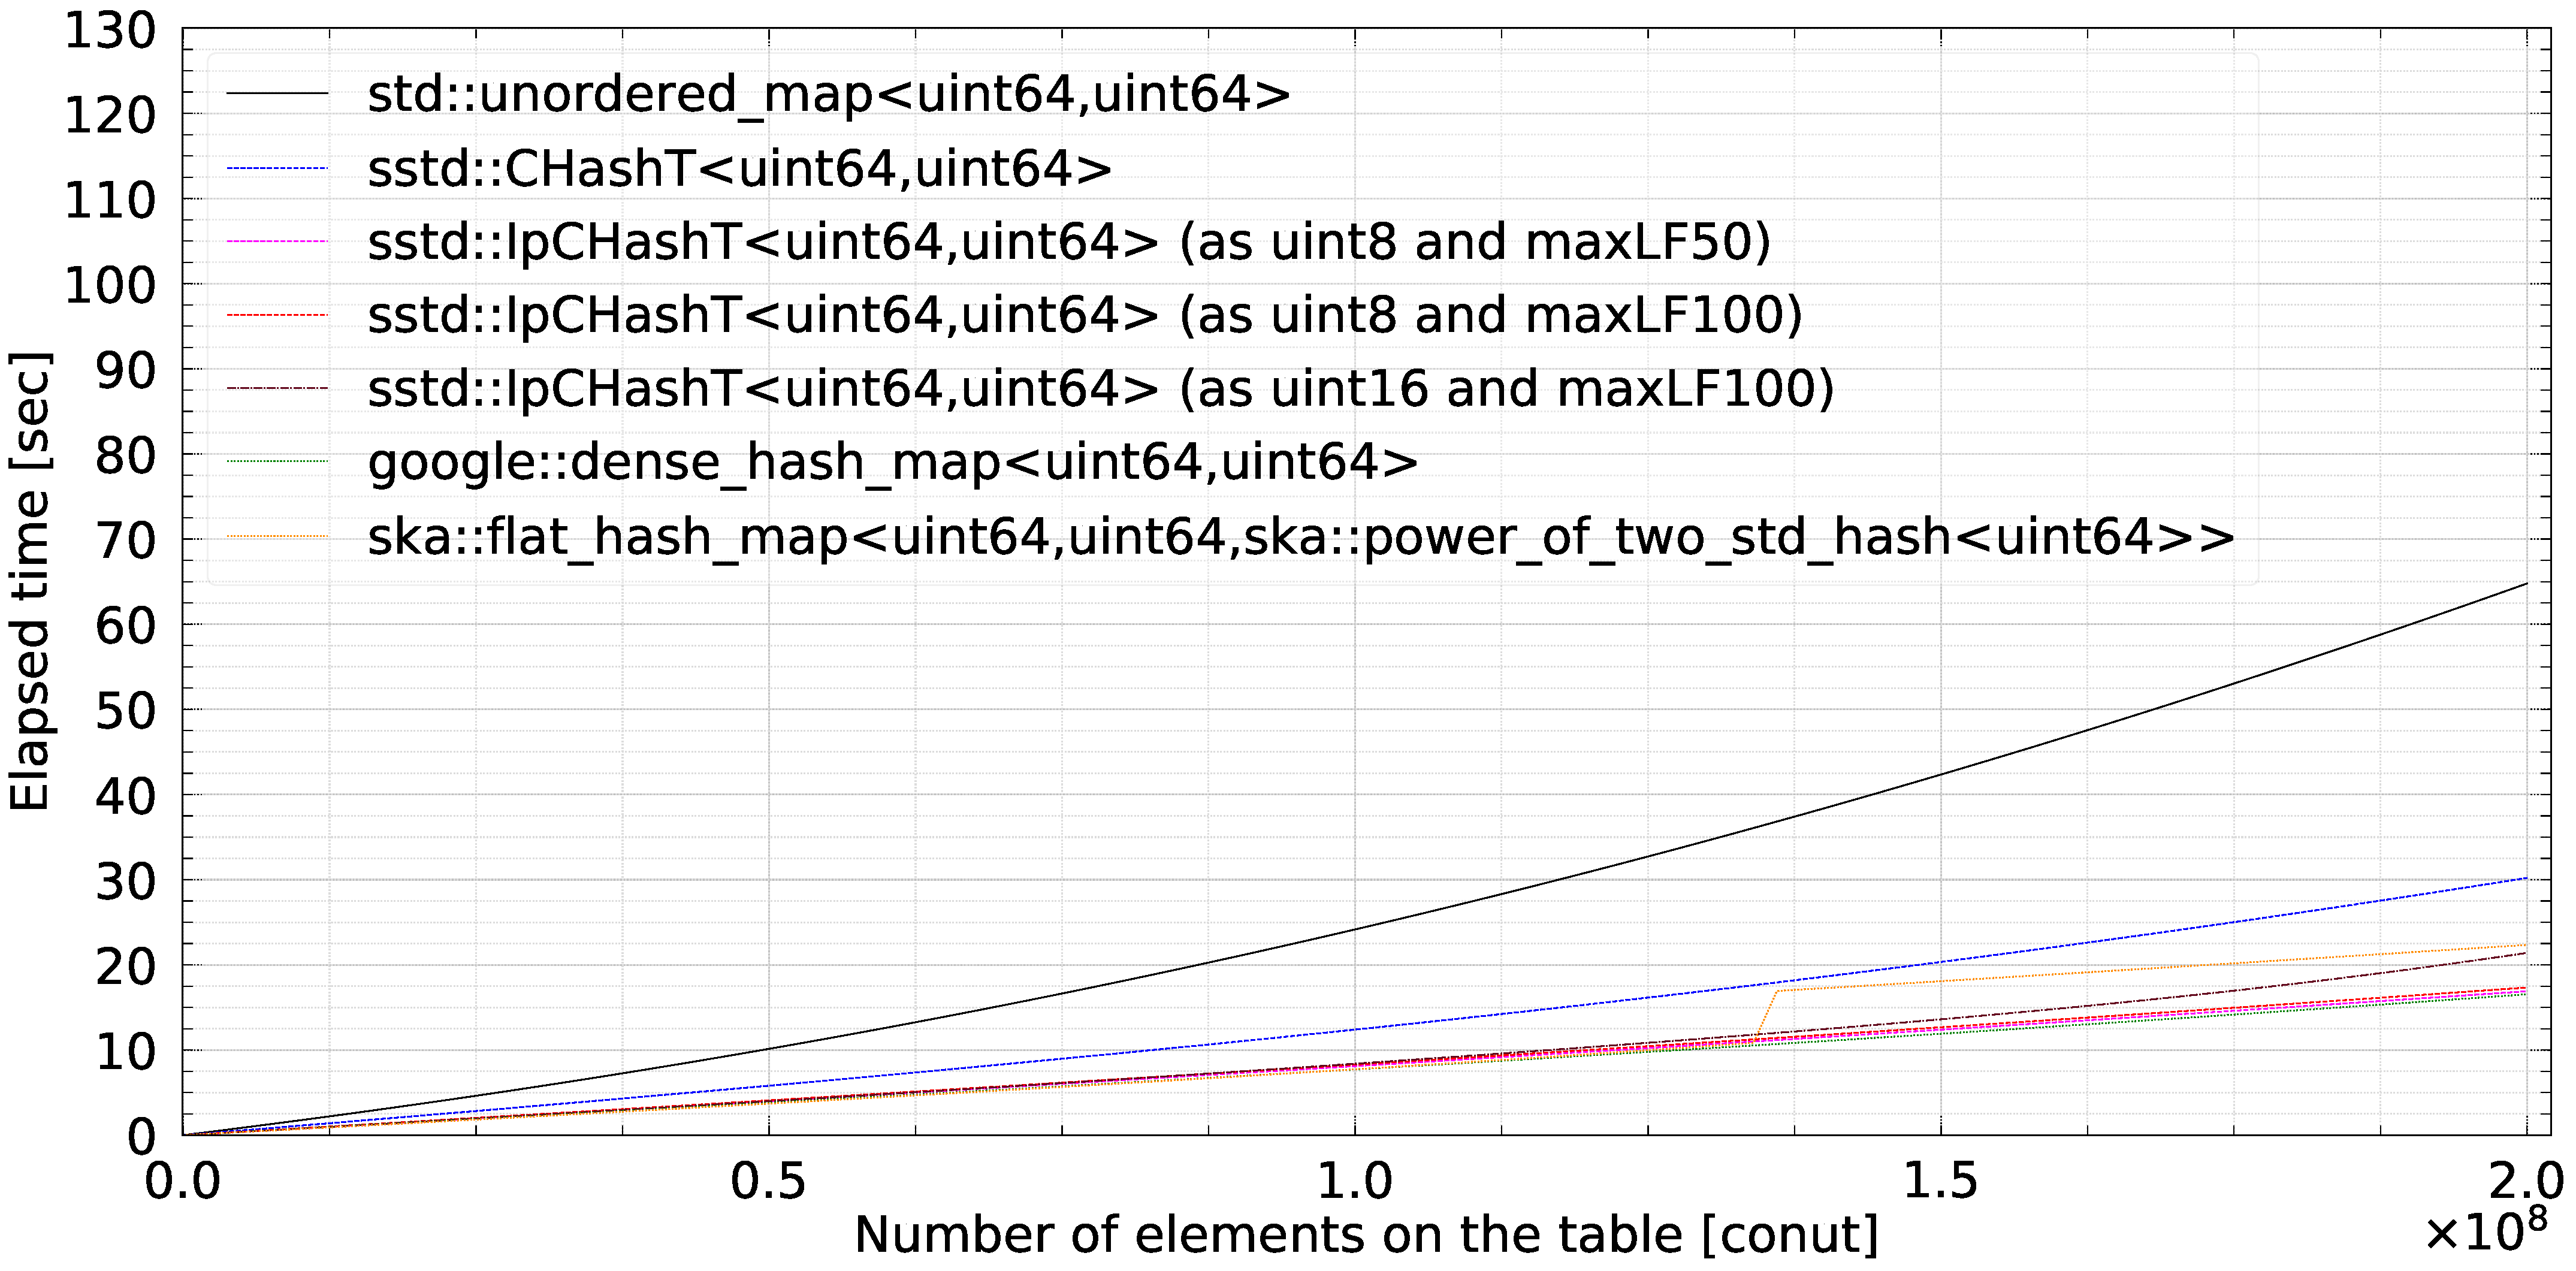
\includegraphics[scale=0.24]{./fig_bench/insert_et_preAlloc_med.pdf}
  \caption{
    Total time of insertion using pre-allocated table which is median value of 100 samples.
    sstd::IpCHash (as maxLF50) and ska::flat\_hash\_map are rehashing around $4.1\textasciitilde.2\times10^6$.
  }
  \label{fig_bench_insert_preAlloc}
\end{figure}

\begin{figure}[h]
  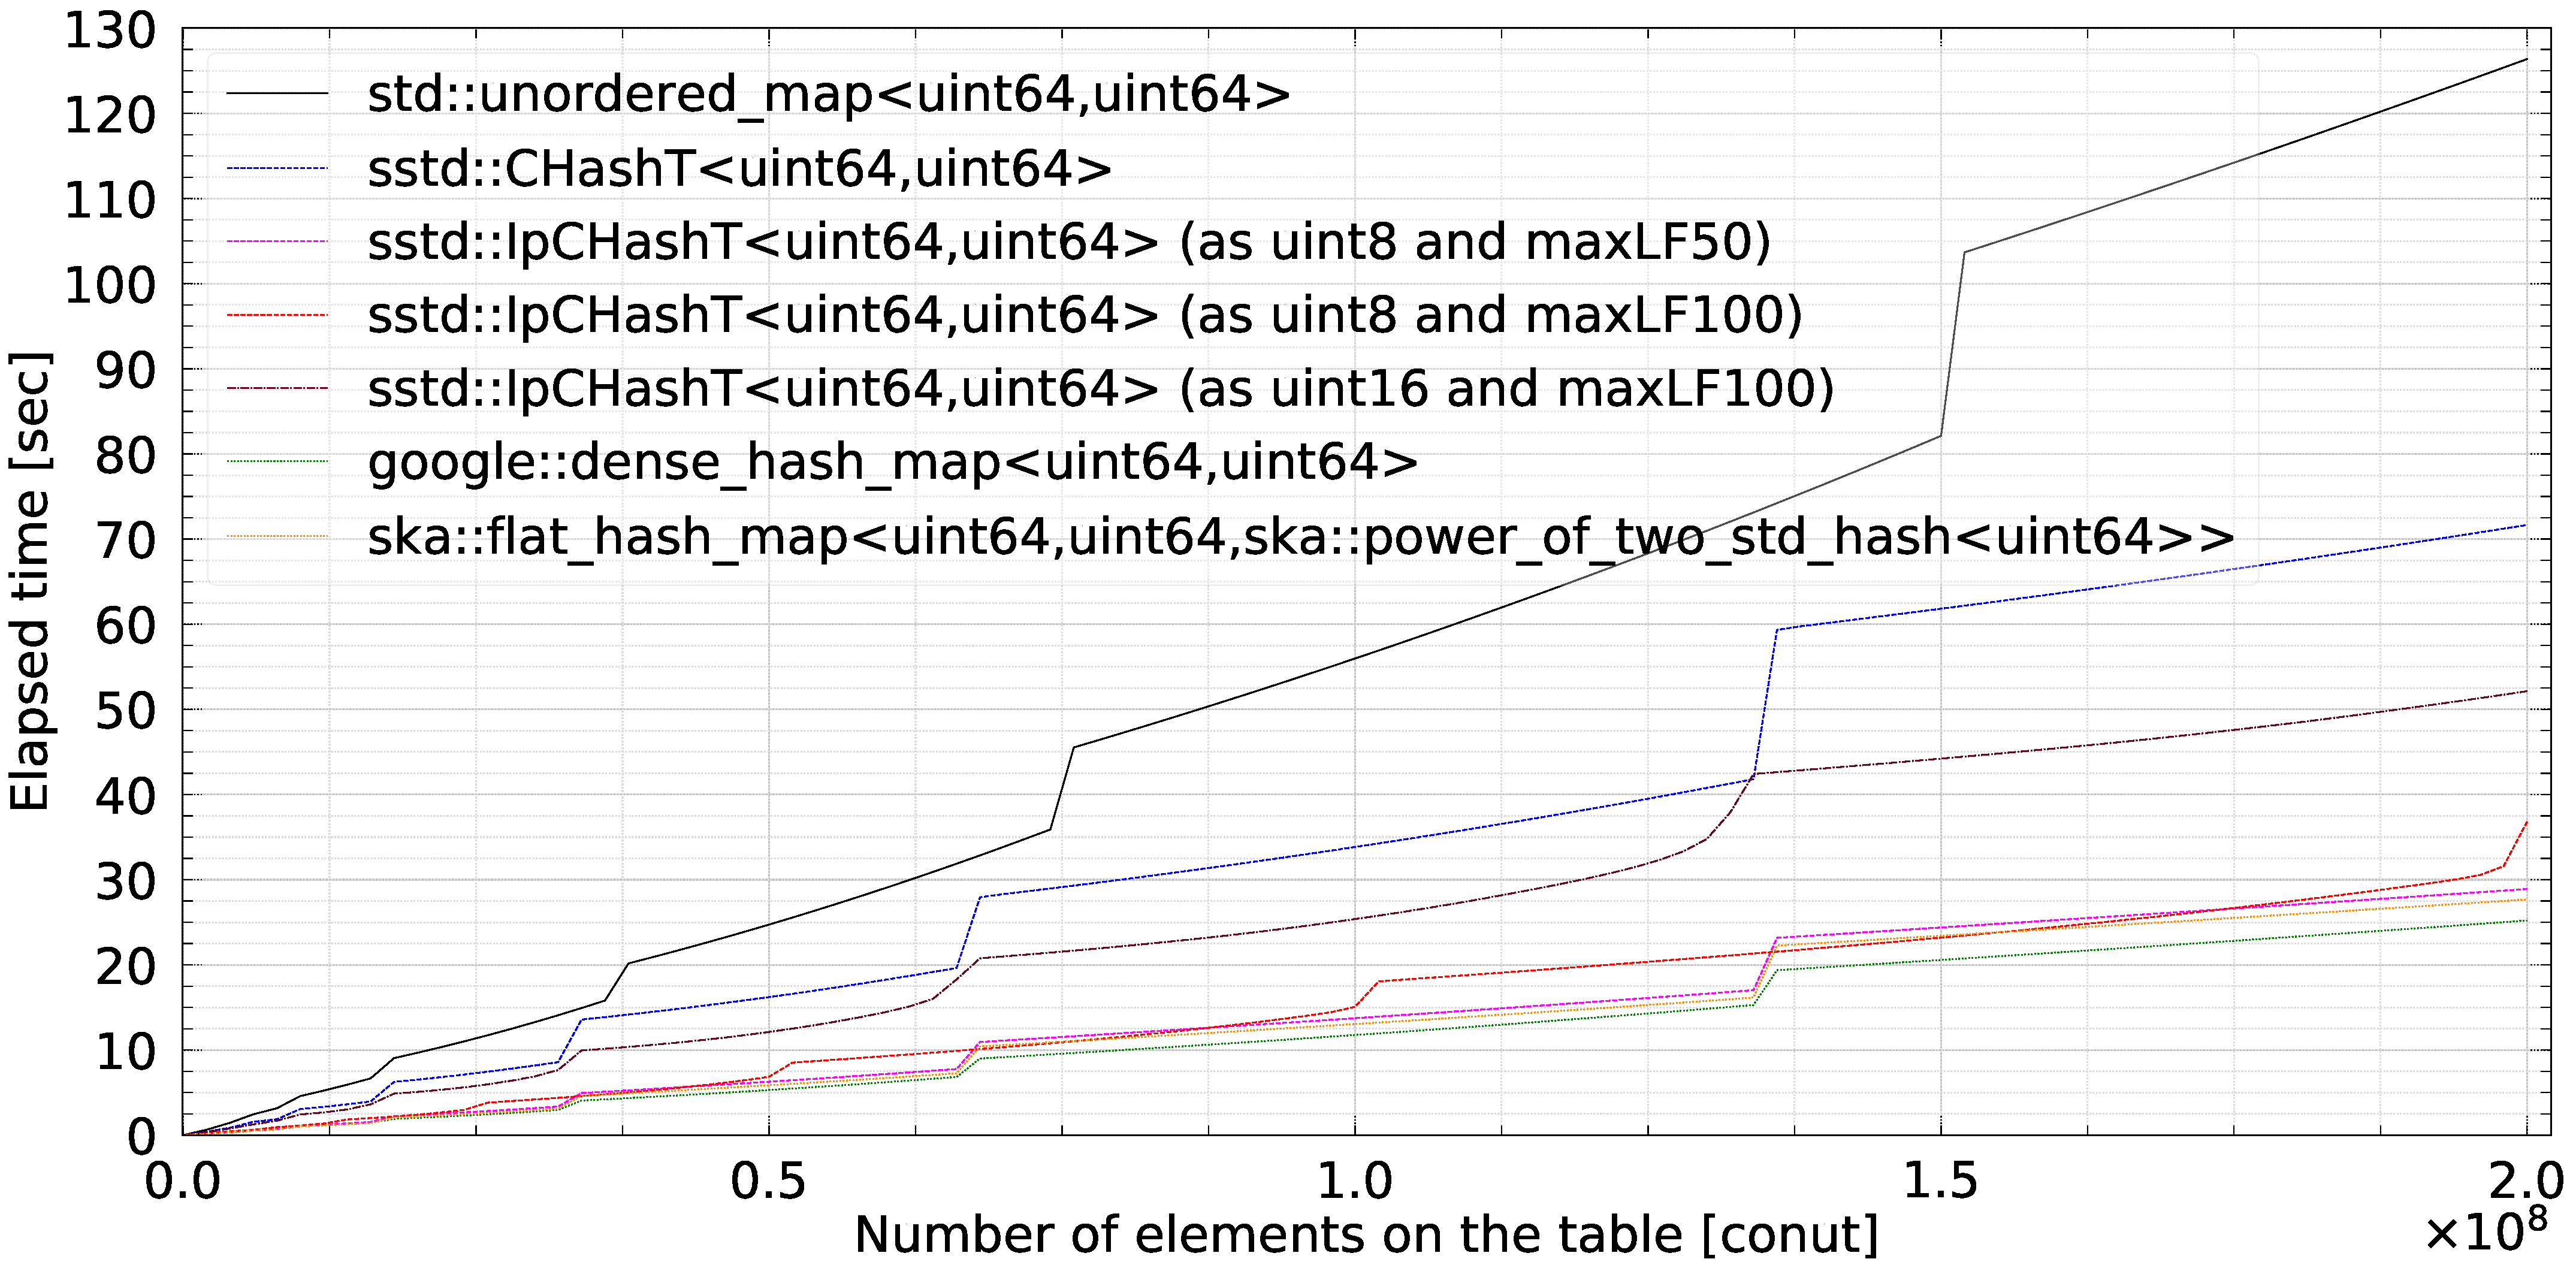
\includegraphics[scale=0.24]{./fig_bench/insert_et_med.pdf}
  \caption{
    Total time of insertion with rehashing table which is median value of 100 samples.
    A distortion in sstd::IpCHashT (as uint8 and maxLF100) around elements count $3.5 \textasciitilde.75\times10^6$ is influenced by the maximum load factor.
    Chaining type of hash tables, sstd::CHashT and sstd::IpCHashT are slow down its insertion speed in high load factor range.
  }
  \label{fig_bench_insert_wRehash}
\end{figure}

\begin{figure}[h]
  \hspace{-3mm}
  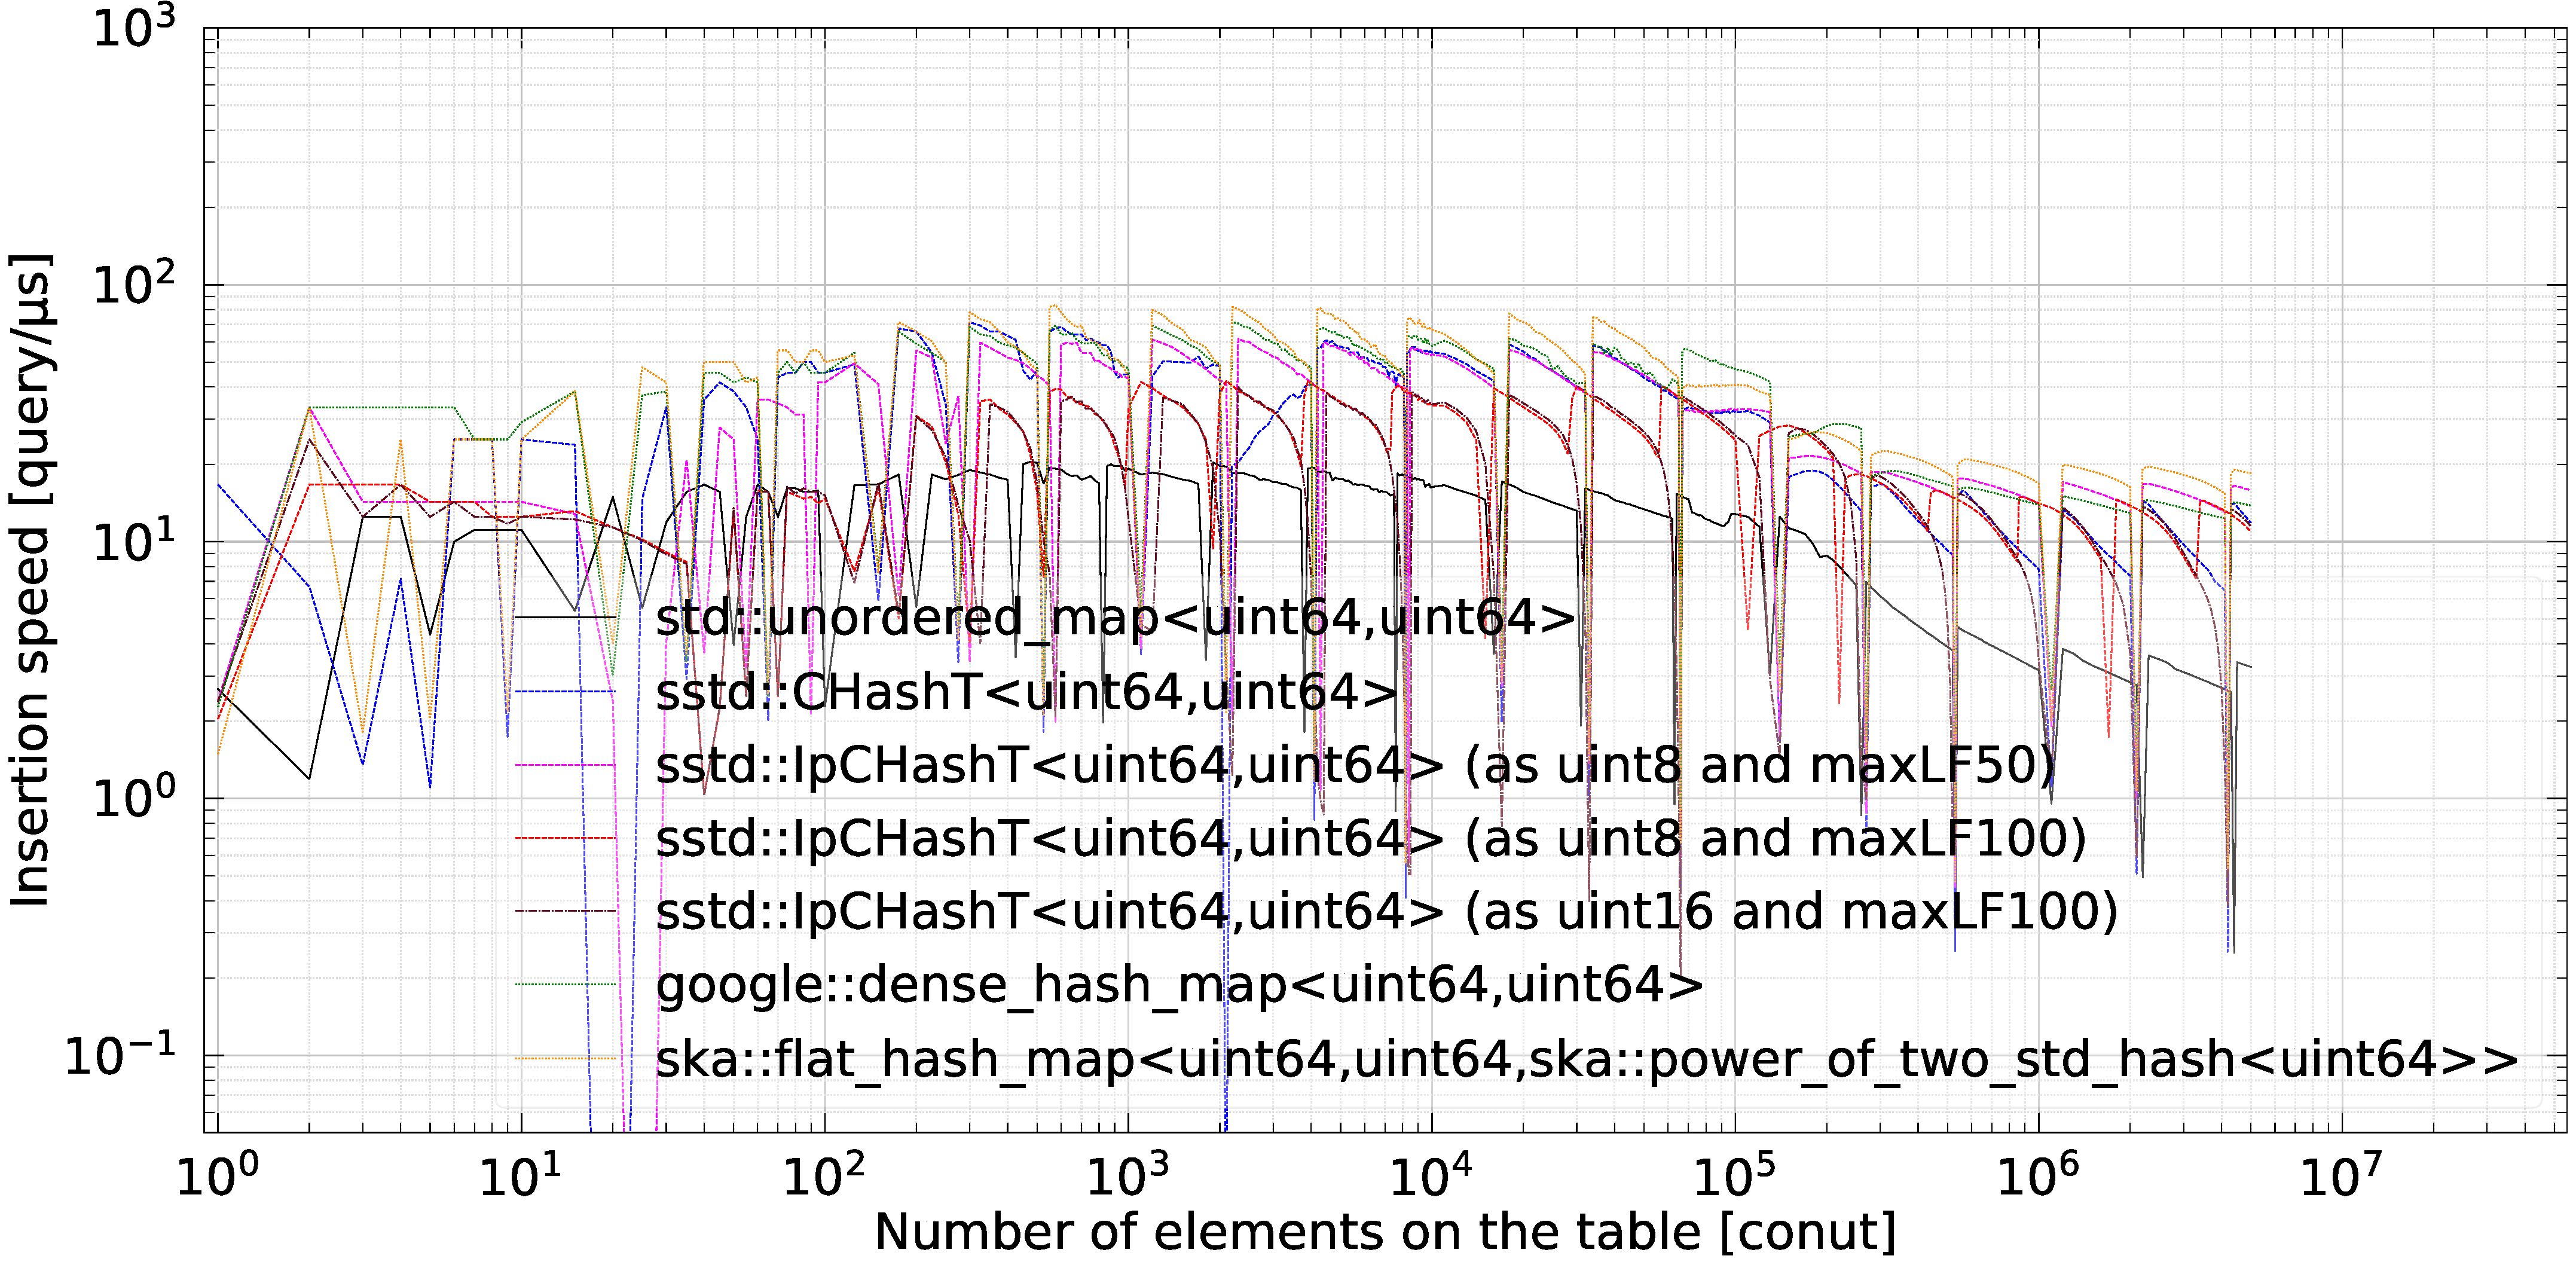
\includegraphics[scale=0.24]{./fig_bench/insert_med.pdf}
  \caption{ Insertion speed. }
  \label{fig_bench_insert}
\end{figure}

\begin{figure}[h]
  \hspace{-3mm}
  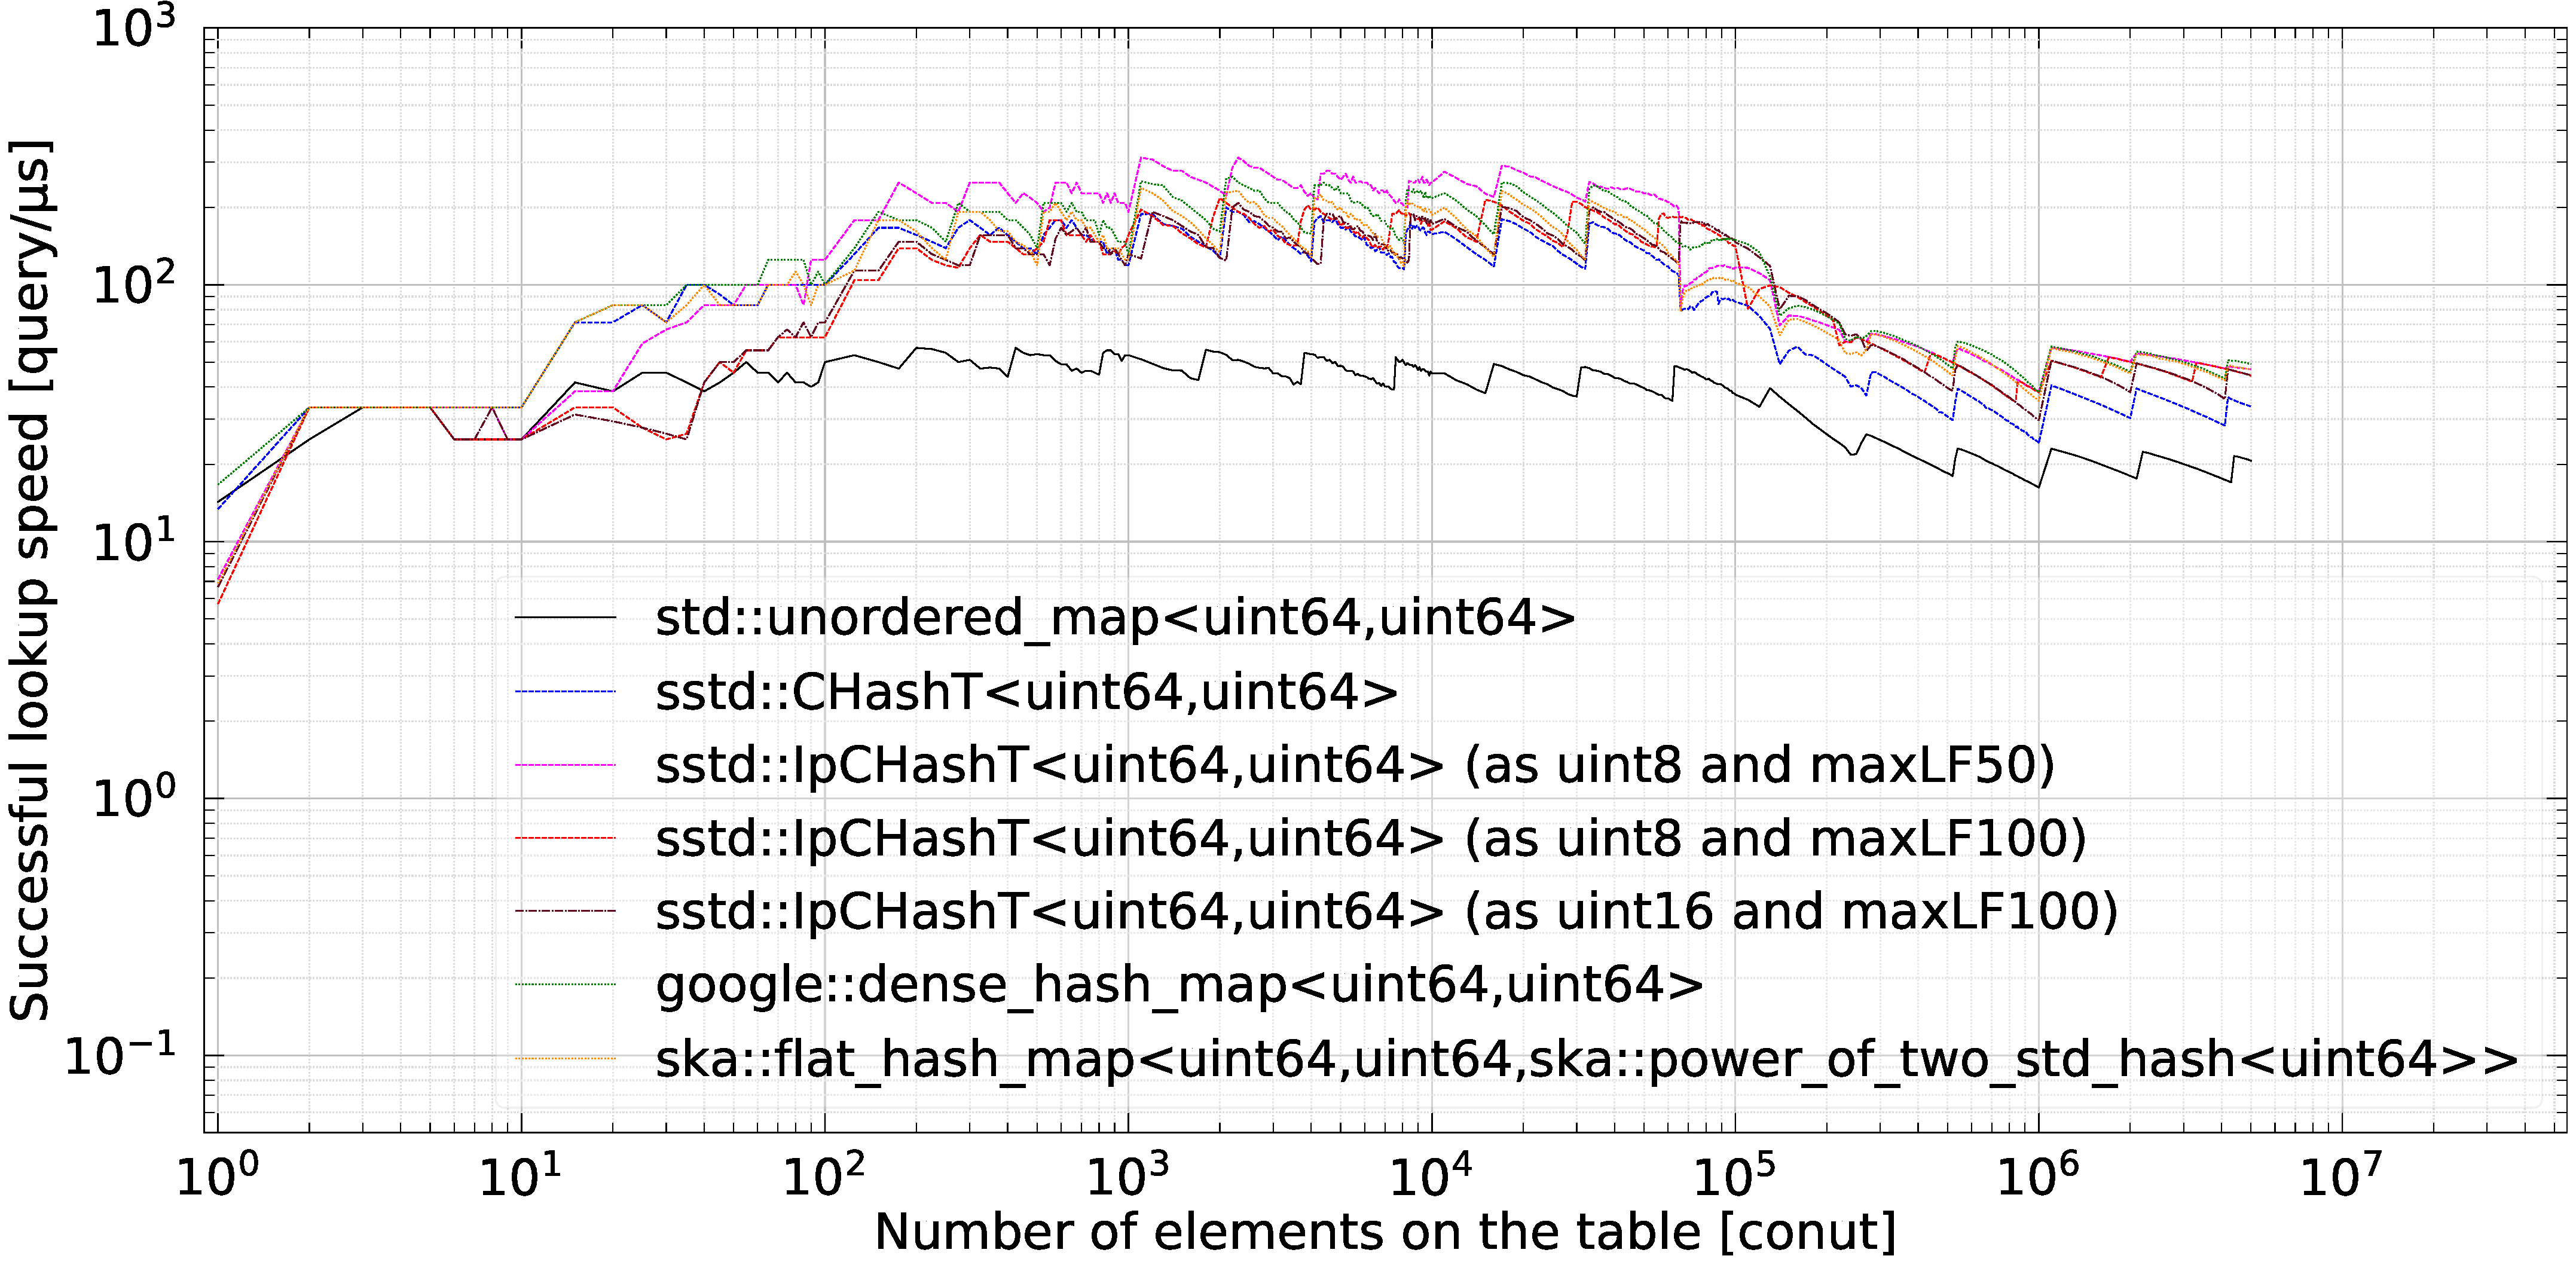
\includegraphics[scale=0.24]{./fig_bench/find_successful_lookup_med.pdf}
  \caption{ Successful lookup speed. }
  \label{fig_bench_insert}
\end{figure}

\begin{figure}[h]
  \hspace{-3mm}
  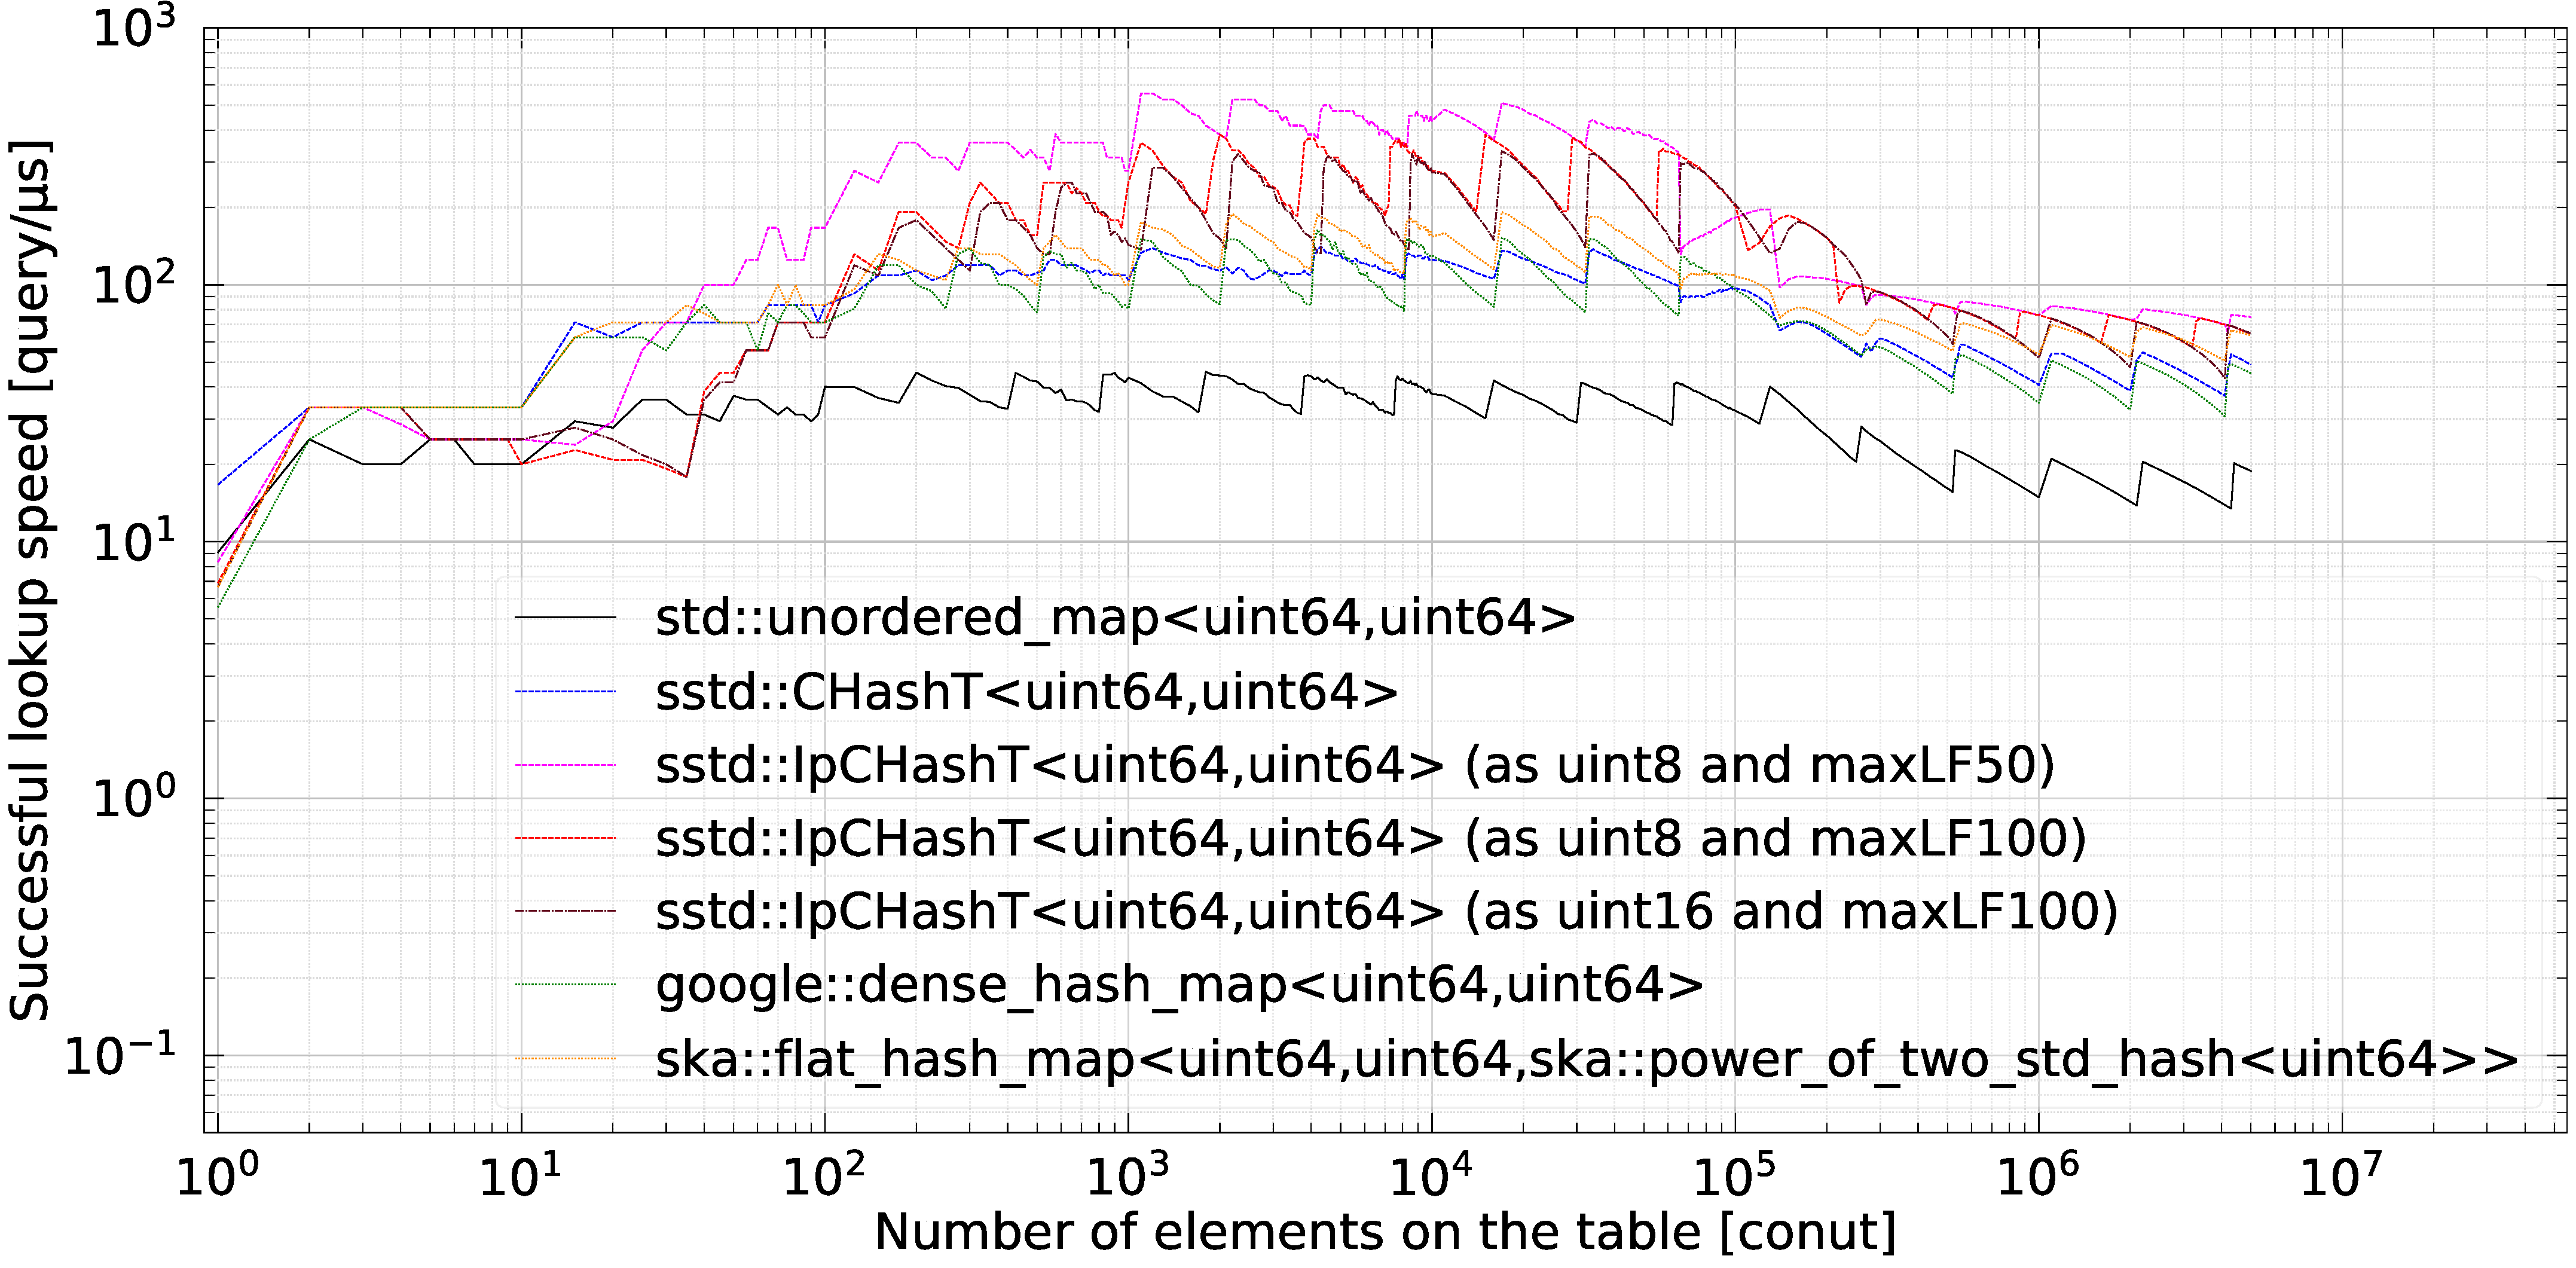
\includegraphics[scale=0.24]{./fig_bench/find_unsuccessful_lookup_med.pdf}
  \caption{ Unsuccessful lookup speed. }
  \label{fig_bench_insert}
\end{figure}

\begin{figure}[h]
  \hspace{-3mm}
  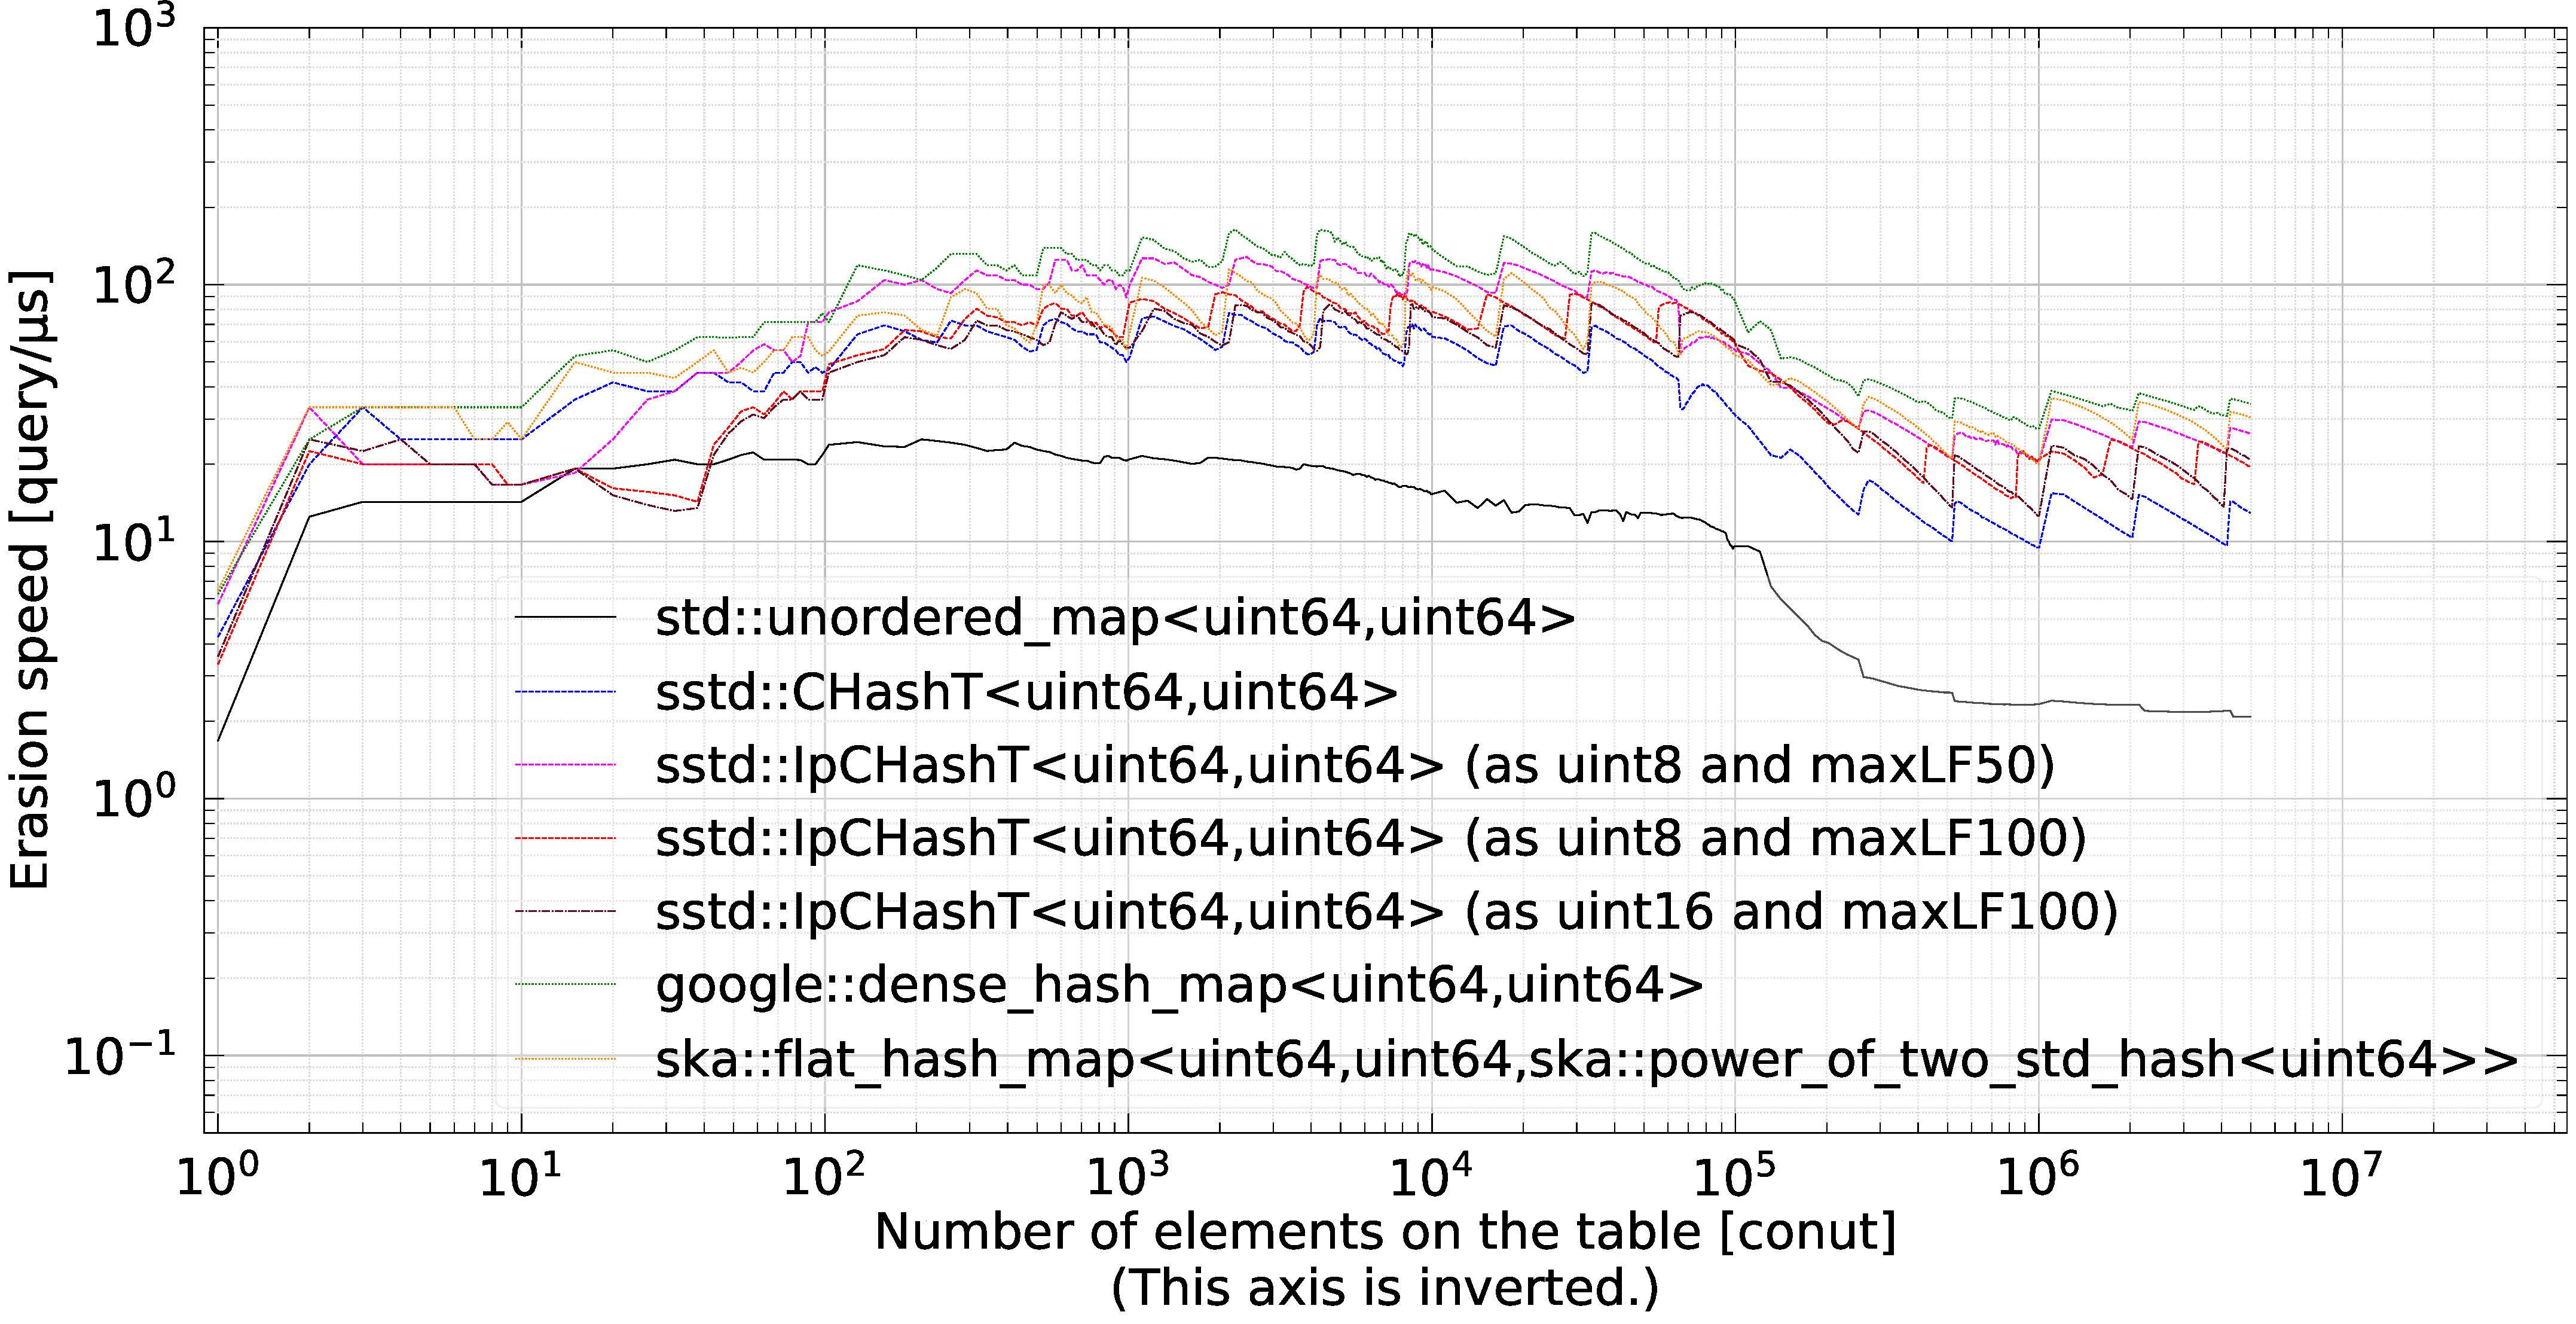
\includegraphics[scale=0.24]{./fig_bench/erase_med.pdf}
  \caption{ Erasion speed. }
  \label{fig_bench_insert}
\end{figure}
















